\chapter{Introduction}
% Tot mai multe persoane au nevoie de recuperare medicala din toate categoriile de varsta.  
% Exista multe cazuri in care apare un o problema medicala care poate fi rezolvata prin recuperare.

More and more people need medical recovery from all age groups.
There are many cases where there is a medical problem that can be resolved by medical recovery.

% De exemplu in cazul persoanelor care sufera anumite accidente si raman paralizate complet sau partial, 
%  recuperarea este vitala in mentineri si imbunatatirea stari persoanei.
% Alte probleme care apar frecvent la orice varsta sunt fracturile care necesita o atentie sporita 
% si un program de recuperare in cele mai multe cazuri.

For example, in the case of people who suffer accidents and remain paralyzed completely or partially, 
recovery is vital in maintaining and improving the person's condition.
Other problems that occur frequently at any age are fractures that require increased attention 
and a recovery program in most cases.

% In cazul persoanelor mai invarsta exista multiple probleme care apar si 
% necesita recuperarea medicala, una dintre probleme este osteoporoza, 
% in jur de 10 milioane de americani au acesta problema iar altele 34 de milioane au probleme cu masa osoasa, 
%  cea ce reprezinta un risc ridicat de aparitie a unei probleme. \cite{keen2003burden}
% Si in cazul copiilor exista un numar semnificativ care sau nascut cu diferite deficite de miscare.

In the case of older people, there are many problems that arise and
require medical recovery, one of the problems is osteoporosis,
around 10 million Americans have this problem and another 34 million have problems with bone mass, 
which is a high risk of a problem.\cite{keen2003burden}
And in the case of children there is a significant number that is born with different deficits of movement.

% Multe persoane negijeaza recuperarea medicala, datorit lipsei progresului sau a costurilor ridicat.
Many people quit medical recovery due to lack of progress or high costs.

% De exemplu in america se cheltuie anual peste 18 miliarde USD datorita accidentarilor persoanelor mai invarsta.  
For example, America spends more than \$18 billion annually on account of injuries to older people
(Burns, Stevens, Lee, 2016; Stevens, Corso, Finkelstein,  Miller, 2006).

\section{Physical Therapy}

% Încă din antichitate (China antică, India antică, Grecia antică, Egiptul antic etc), 
% exerciţiile fizice erau practicate pentru 
% menţinerea unei bune forme fizice, dar şi în tratarea unor afecţiuni cum ar fi dureri musculare,
%  guta, obezitate etc.
Ever since antiquity (ancient China, ancient India, ancient Greece, ancient Egypt, etc.), 
physical exercises have been practiced to maintain a good physical
form but also to treat diseases such as muscular pain, gout, obesity, etc.

% Marele medic al antichităţii greceşti, Hipocrat , în primul spital 
% construit în insula Kos, a studiat atent efectele fiziologice ale gimnasticii şi
% masajului definind sănătatea ca un echilibru între exerciţiile fizice şi alimentaţie.
% Pentru prima dată este sesizată relaţia între mişcare-hipertrofie şi imobilizare-atrofie musculară.
% El susţine că exerciţiul fizic şi masajul influenţează favorabil respiraţia, metabolismul, 
% circulaţia sangvina şi echilibrează activitatea sistemului nervos central.

The great Greek antiquity doctor, Hippocrates, in the first hospital built on the island of Kos, 
carefully studied the physiological effects of gymnastics and massage defining health as a
 balance between exercise and nutrition. For the first time, the relationship between motion-hypertrophy and 
 immobilization-muscular atrophy is noted. He argues that physical exercise and massage influence favorably 
 the breathing, metabolism, blood circulation and balances the activity of the central nervous system. \cite{book.history.rehab.1991}


%  Kinetoterapia se foloseşte pentru recuperarea medicală somato-funcţională şi 
%  constă într-un ansamblu de tehnici şi metode având în centru exerciţiul fizic.
 Physical therapy is used for somato-functional medical recovery and 
 consists of a set of techniques and methods that center the physical exercise.

% În cadrul Kinetoterapiei sunt cuprinse trei forme de kinetoprofilxie: primară, secundară şi terţiară.
 Physical therapy includes three forms of kinetoprophylaxis: primary, secondary, and tertiary.

\begin{itemize}
  \item Primary when using physical exercise, techniques and methods to prevent illness.
  \item Secondary kinetoprophylaxis has the role of preventing complications of illnesses.
  \item Tertiary kinetoprophylaxis prevents the appearance of sequelae following illnesses that could cause motor disabilities.
\end{itemize}

% Principalele obiective ale kinetoterapiei sunt: relaxarea, creşterea capacităţii de efort, 
% creşterea forţei, rezistenţei musculare si corectarea posturii.

The main goals of physical therapy are relaxation, increased exercise capacity, 
increased strength, muscle strength and posture correction.

% Dezvoltările tehnologice actuale au permis utilizarea tehnologiilor computerizate 
% în kinetoterapie pentru diferite masuratori, 
% permiţând evaluarea precisă şi personalizarea tratamentului.
Current technological developments have allowed the use of computer technologies in physiotherapy
 for different measurements, allowing accurate assessment and treatment personalization.
\section{Track progress in rehabilitation therapy}


\par In Physiotherapy, tracking Range of Motion (ROM) is a standard approach to measuring progress in patient therapy. 
Often, ROM is measured subjectively and documentation is inconsistent between clinicians. 
Physios might come to wrong conclusions if ROM is tracked incorrectly between therapy sessions.


\par The problem is that up to 70\% of patients give up physiotherapy because they can not see 
immediate results \cite{7FactsInPhysicalTherapy}.
\par That's why we want to make a application which makes use of a camera to objectively 
calculate ROM in real-time and automatically produce a report that tracks progress over the course 
of several therapy sessions.

\begin{figure}[htbp]
	\centerline{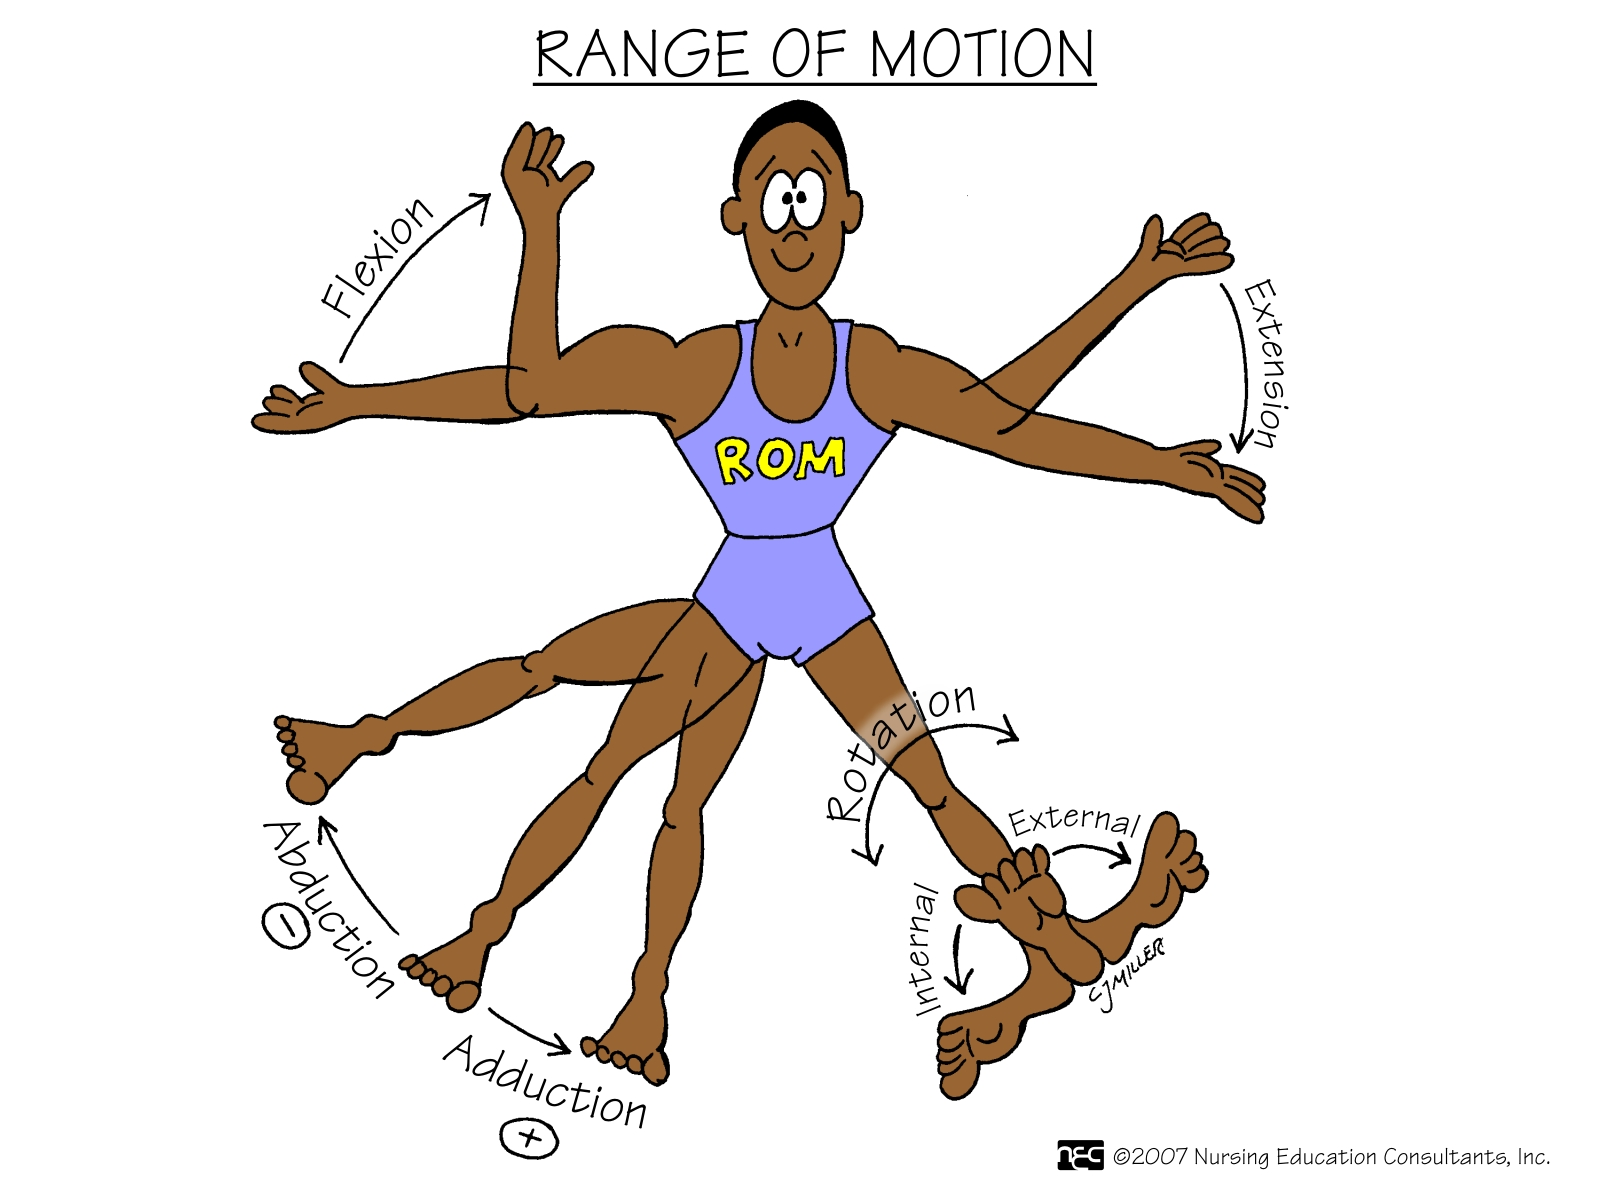
\includegraphics[scale=0.25]{fig/rangeofmotion.png}}  
	\caption{Range of Motion}
\end{figure}

\section{What is pose estimation?}